\documentclass{tufte-handout}

\title{Probability and z-scores}


%\author[The Tufte-LaTeX Developers]{The Tufte-\LaTeX\ Developers}

\date{} % without \date command, current date is supplied


\usepackage{graphicx} % allow embedded images
  \setkeys{Gin}{width=\linewidth,totalheight=\textheight,keepaspectratio}
  \graphicspath{{graphics/}} % set of paths to search for images
\usepackage{amsmath}  % extended mathematics
\usepackage{booktabs} % book-quality tables
\usepackage{units}    % non-stacked fractions and better unit spacing
\usepackage{multicol} % multiple column layout facilities
\usepackage{lipsum}   % filler text
\usepackage{fancyvrb} % extended verbatim environments
  \fvset{fontsize=\normalsize}% default font size for fancy-verbatim environments

\usepackage{pgfplots}
\pgfplotsset{compat=1.12}

% Standardize command font styles and environments
\newcommand{\doccmd}[1]{\texttt{\textbackslash#1}}% command name -- adds backslash automatically
\newcommand{\docopt}[1]{\ensuremath{\langle}\textrm{\textit{#1}}\ensuremath{\rangle}}% optional command argument
\newcommand{\docarg}[1]{\textrm{\textit{#1}}}% (required) command argument
\newcommand{\docenv}[1]{\textsf{#1}}% environment name
\newcommand{\docpkg}[1]{\texttt{#1}}% package name
\newcommand{\doccls}[1]{\texttt{#1}}% document class name
\newcommand{\docclsopt}[1]{\texttt{#1}}% document class option name
\newenvironment{docspec}{\begin{quote}\noindent}{\end{quote}}% command specification environment


\begin{document}

\maketitle% this prints the handout title, author, and date


%\printclassoptions

\section{Probability Basics}
\begin{marginfigure}
  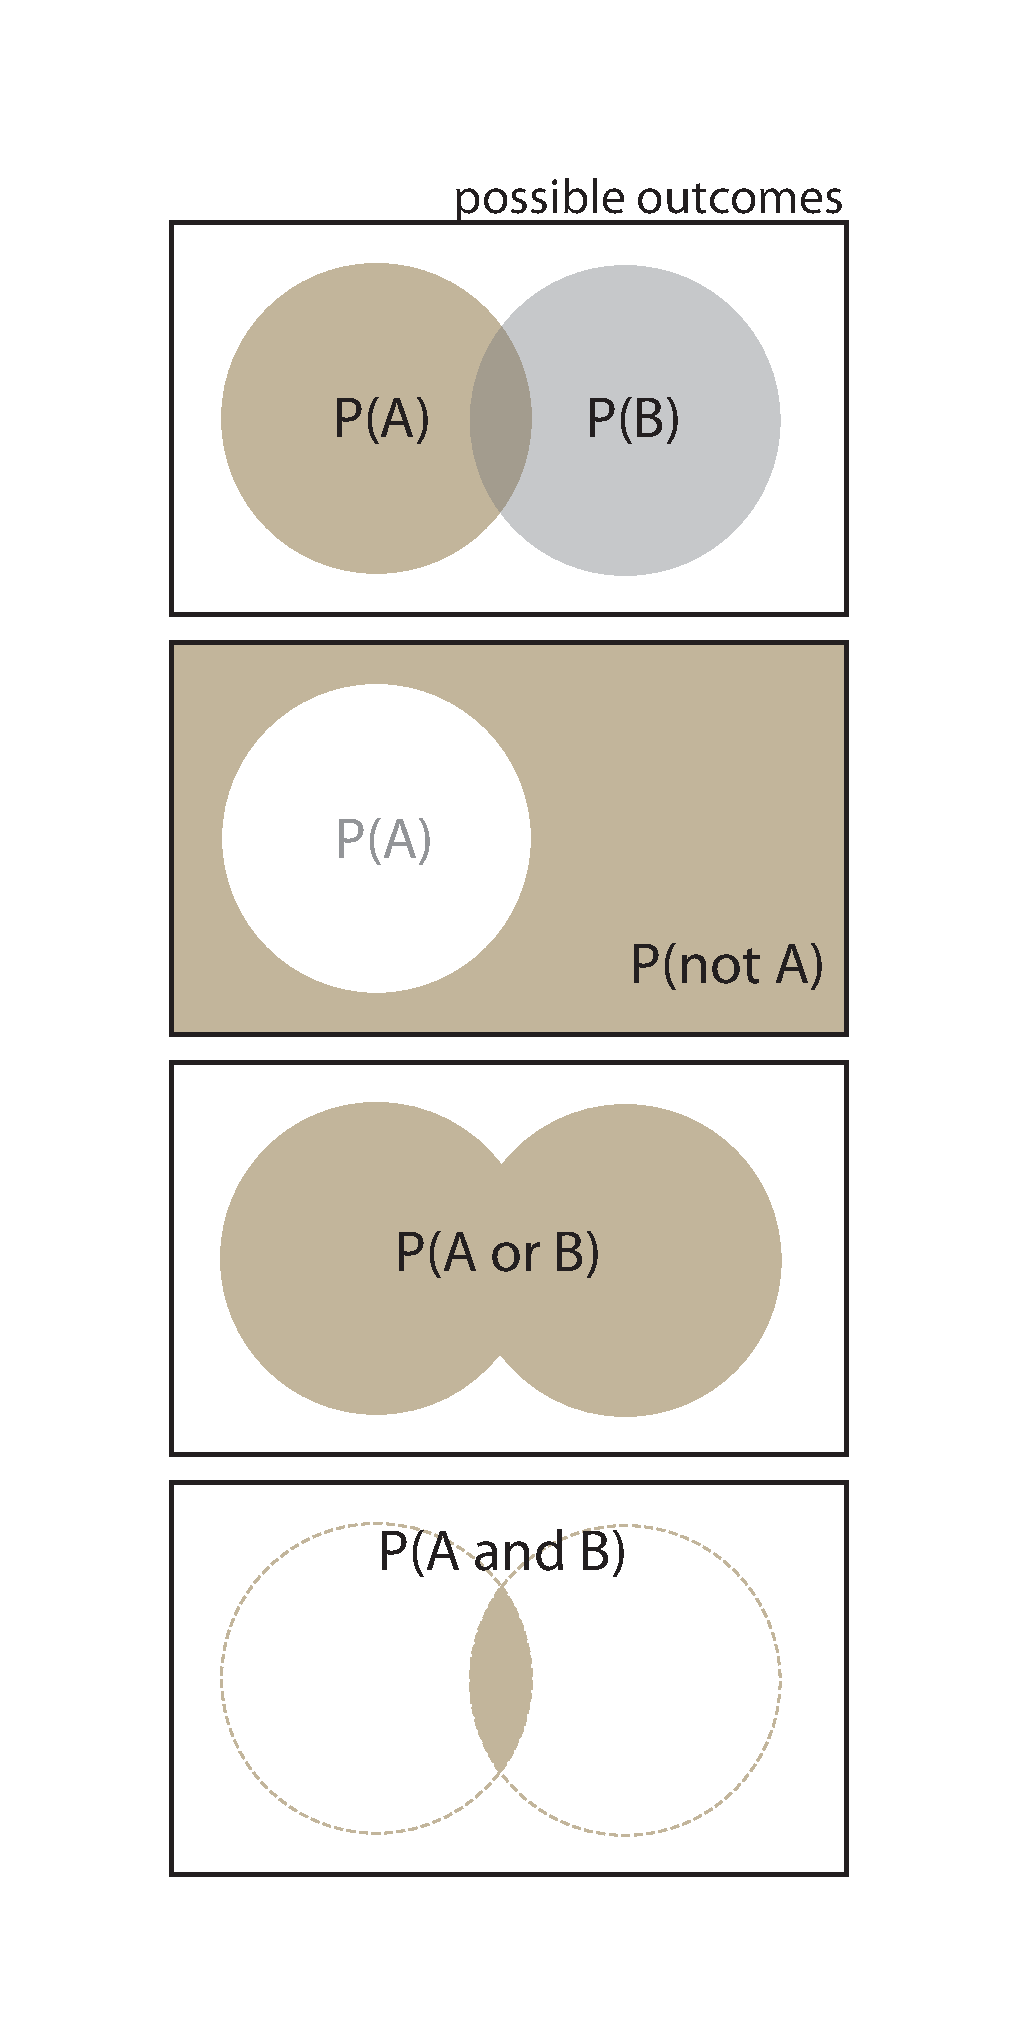
\includegraphics[width=\linewidth]{handout2_probability}%
  \label{fig:fullfig}%
  \setfloatalignment{t}
  \caption{Visual probability rules.}
\end{marginfigure}
\begin{equation*}
P(A)=\frac{\text{number of times } A \text{ occurs}}{\text{number of possible outcomes}}
\end{equation*}
Probability Rules:
\begin{equation*}
P(A)=1-P(\text{not } A)
\end{equation*}
\begin{equation*}
P(A \text{ or } B)=P(A)+P(B)-P(A \text{ and } B)
\end{equation*}
If the events are independent...
\begin{equation*}
P(A \text{ and } B)=P(A)P(B)
\end{equation*}
In general...
\begin{equation*}
P(A \text{ and } B)=P(A|B)P(B)
\end{equation*}
Where $p(A|B)$ is the probability of event $A$ given that event $B$ occurred. It's important to remember that 1) probabilities always sum to 1, and 2) probability can also be thought of as an area under a distribution.

\section{z-scores}
\begin{margintable}[80pt]
  \centering
  \fontfamily{ppl}\selectfont
  \begin{tabular}{rrr}
    \toprule
    $z$ & $p(-z \leq x\leq z)$ &\\
     1  &   0.683\\
     2 &   0.955\\
     3 &   0.997\\
    \midrule
    $z$ & $p(x\leq z)$ &\\
     1.645  &   0.950\\
     2.326 &   0.990\\
     3.901 &   0.999\\
    \bottomrule
  \end{tabular}
  \label{tab:normaltab}
\end{margintable}
z-scores are a way of standardizing from different distributions.
\begin{align*}
&\text{Population z-score:} & z&=\frac{X-\mu}{\sigma}\\
&\text{Sample z-score:} & z&=\frac{X-\bar{X}}{s}
\end{align*}
If $X$ follows a normal distribution then the z-scores follow a \emph{standard normal distribution} (the normal distribution with mean $\mu=0$ and standard deviation $\sigma=1$), and probabilities for any interval of the distribution can be looked up using the standard normal table.
\begin{figure*}[h]
  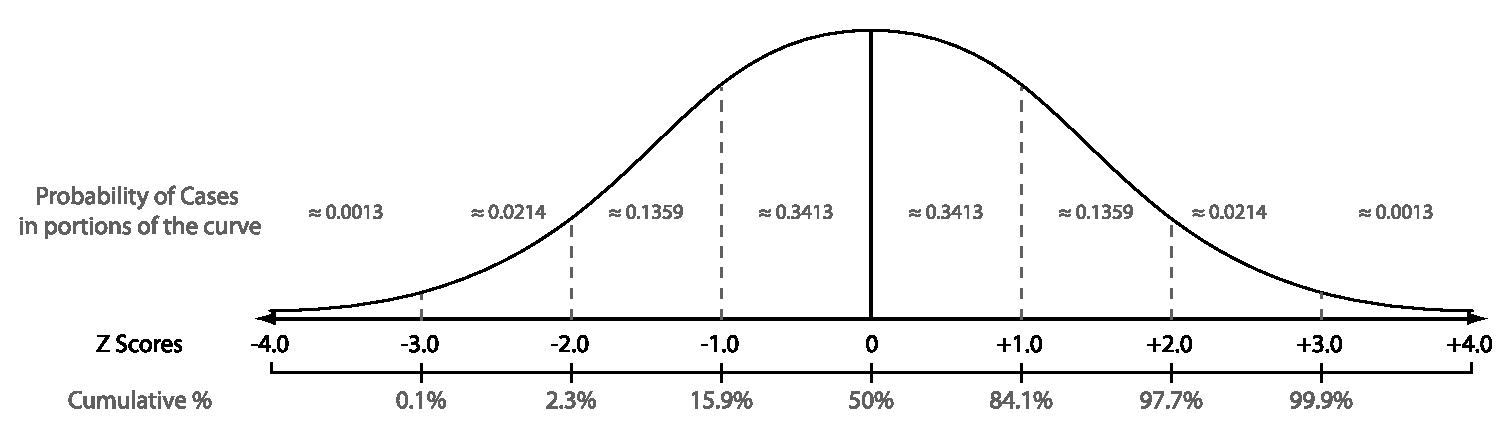
\includegraphics[width=\linewidth]{handout2_standard_normal}%
  \label{fig:fullfig}%
  \caption{Standard Normal Distribution with mean $\mu=0$ and standard deviation $\sigma=1$. z-scores measure deviations from the mean in units of standard deviations.}
\end{figure*}

\pagebreak

\section{Distribution of Sample Means}
In many cases, instead of comparing single scores, we want to summarize the entire sample and compare the average outcome to some known quantity. Since samples vary, we need a way to think about how certain we are about the sample mean. What would we expect if we ran the same experiment again? The answer is that we would get the distribution of sample means, which has two key properties

\begin{description}
\item[1.] The mean and standard deviation are related to the population parameters with $\mu_M = \mu$ and $\sigma_M=\sigma/\sqrt{n}$.
\item[2.] Surprisingly, no matter what the shape of the population is, the distribution of sample means becomes normal for $n > 30$.
\end{description}

The purpose of this distribution is to describe the expected variation in the mean due to chance sampling error.

\section{The z test (one-sample location test)}
Describing \emph{what happens by chance} is the key to all of hypothesis testing. Suppose, we want to make a decision about whether the mean of our data is significantly different from some known value. Assuming that the population is normal or $n > 30$ and that $\sigma$ is known, the distribution of sample means exactly describes what we expect. After calculating a test statistic $z=\frac{\bar{X}-\mu}{\sigma_M}$ we can look up a probability (p-value) for how extreme such a result would be in a standard normal table.
\begin{figure}
  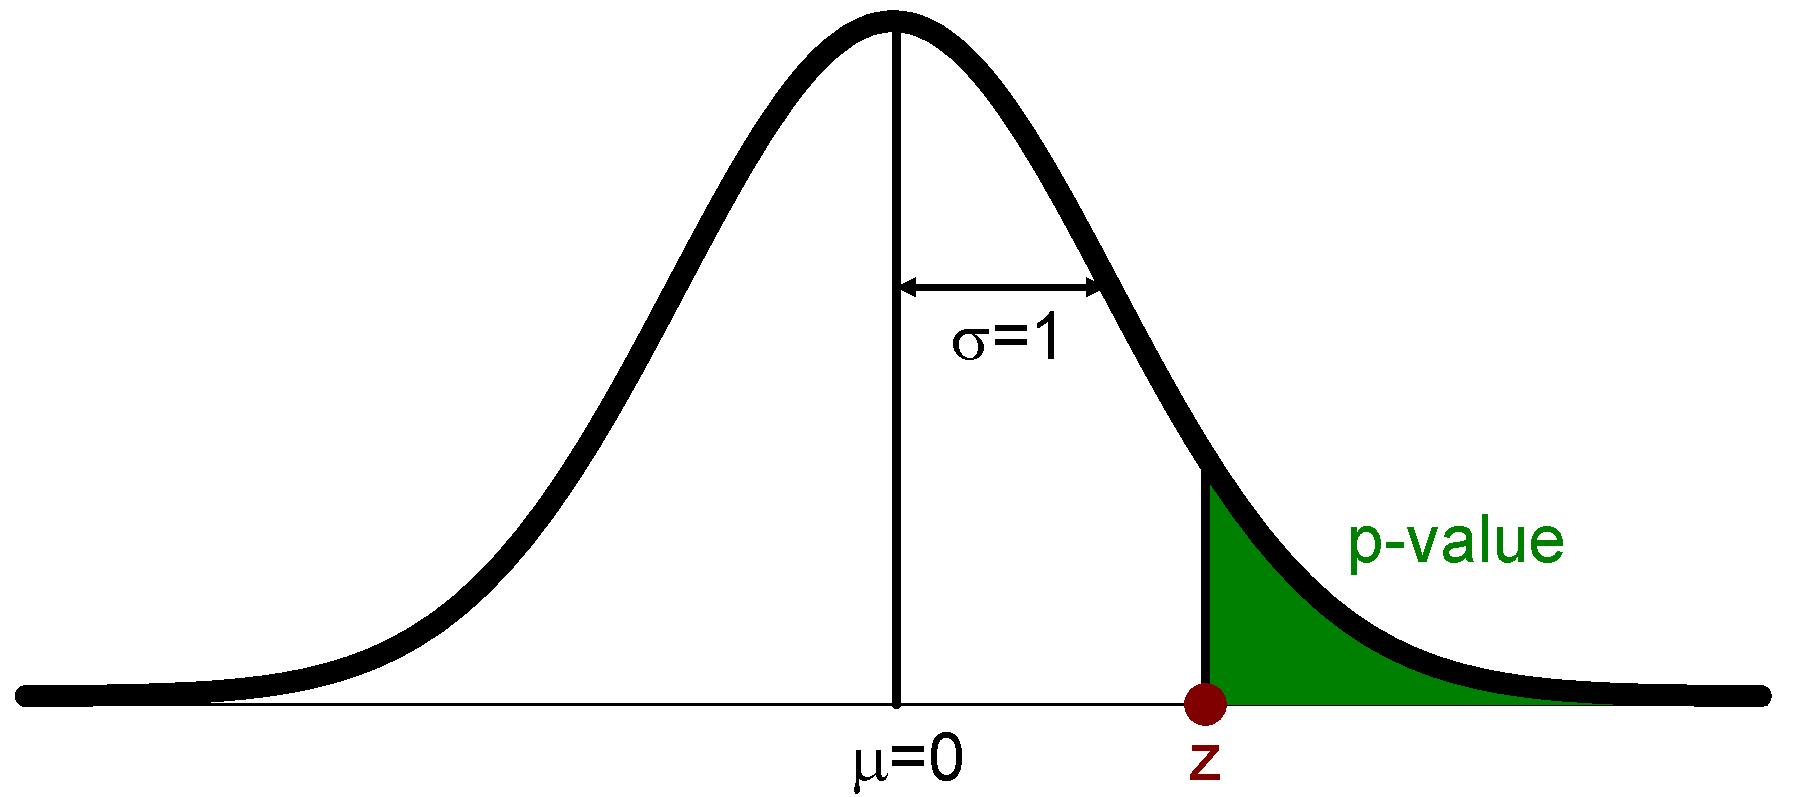
\includegraphics[width=275pt]{handout2_ztest}%
  \label{fig:fullfig}%
  \caption{Illustration of a one-tailed z-test. The p-value (shaded) is the probability of getting a result that is as extreme or more extreme than the test statistic (assuming the null hypothesis is true).}
\end{figure}

In almost all real world situations we don't know the parameters of the population. Instead, we estimate $\sigma_M$ using the \emph{standard error of the mean}:
\begin{equation*}
SEM=\frac{s}{\sqrt{n}}
\end{equation*}					 
Errorbars are commonly reported/plotted using $\bar{X}\pm SEM$.

\end{document}
